% Source: http://www.brian-amberg.de/uni/poster/
\documentclass[landscape,specialSize,fontscale=0.3]{./poster/poster}
\usepackage[vlined]{./poster/poster}
\usepackage{times,calc}
\usepackage{amsmath,amssymb}
\usepackage{relsize}
\usepackage{multirow,multicol}
\usepackage[T1]{fontenc}
\usepackage{ae}
\usepackage{url}

\usepackage{enumitem}\setlist{nolistsep}
\usepackage{graphicx}\graphicspath{{images/}}

\setlength{\columnsep}{0.7em}\setlength{\columnseprule}{0mm}
\newcommand{\compresslist}{
  \setlength{\itemsep}{1pt}
  \setlength{\parskip}{0pt}
  \setlength{\parsep}{0pt}
}

\definecolor{maroon}{cmyk}{0,.8276,.3966,.5451}

\begin{document}
\begin{poster}{
  grid=false, % Show grid to help with alignment
  colspacing=0.7em, % Column spacing
  headerColorOne=maroon, borderColor=maroon, % Color style
  textborder=faded, % Format of textbox
  % Format of text header
  headerborder=open, headershape=roundedright,
  headershade=plain, headerFontColor=white,
  background=none, bgColorOne=white,
  headerheight=0.12\textheight
}{
  %\includegraphics[width=0.06\linewidth]{android-maroon}
}{
  \sc\Huge Title of your project.
}{
  \bigskip\large
  \begin{minipage}{0.3\textwidth}
    Research Symposium \\
    Virginia Tech, April 2014
  \end{minipage}
  \begin{minipage}{0.3\textwidth}
    {\bf Student:} Brandon Amos \\
    Dept. of Computer Science
  \end{minipage}
  \begin{minipage}{0.3\textwidth}
    {\bf Advisor:} Dr. X Y \\
    Dept. of Computer Science
  \end{minipage}
}{
  
\includegraphics[height=0.05\textheight]{./poster/vtlogo-new}
}

\headerbox{Introduction and Motivation: TODO}
    {name=intro,column=0,row=0,span=2}{
  \begin{itemize}
    \item A
    \item B
    \item C
    \item D
    \item E
  \end{itemize}
}

\headerbox{Contribution: TODO}
    {name=contribution,column=0,below=intro,above=bottom}{
  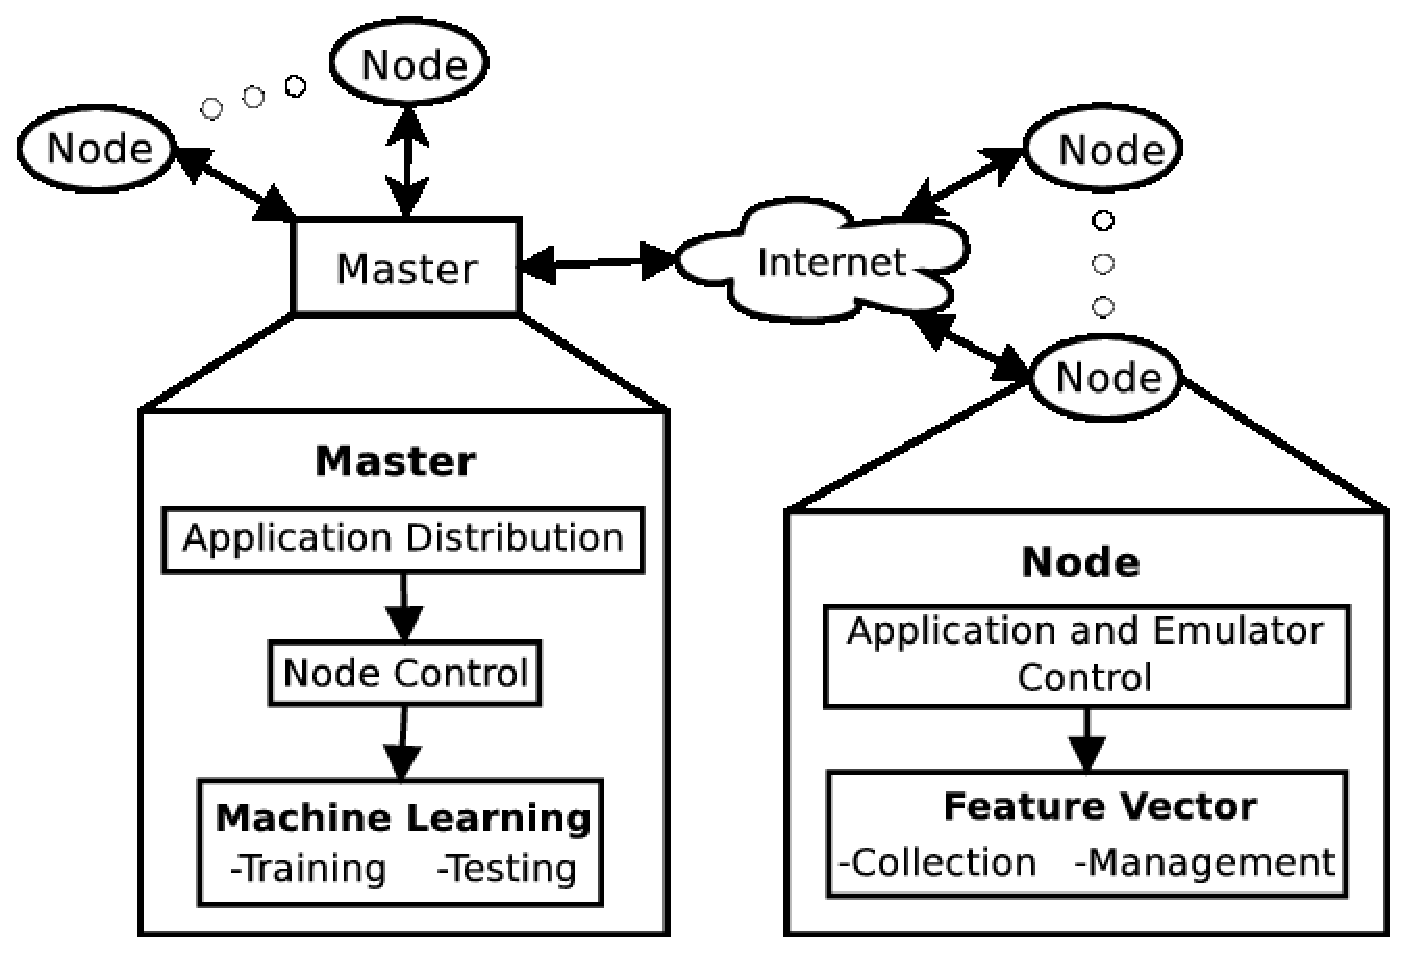
\includegraphics[width=\linewidth]{./poster/stream}
  \begin{itemize}
    \item A
    \begin{itemize}\item A1 \item A2 \item A3\end{itemize}
    \item B \item C \item D \item E
  \end{itemize}
}

\headerbox{TODO {\it Algorithm}}
    {name=algorithm,column=1,below=intro}{
  \begin{algorithm}[H]
      \dontprintsemicolon
      \linesnumbered
      \nl applications.distributeToNodes \;
      \For{node $\in$ nodes}{
          \nl node.applications.distributeToDevices \;
          \For{application $\in$ node.devices.applications}{
              \nl a.install(application) \;
              \nl a.class $\gets$ s.detectClass \;
              \nl a.startDataCollection \;
              \nl a.initializeMonkey \;
              \While{monkey.isRunning}{
                  \nl a.collectFeatureVector \;
              }
              \nl s.featureVector $\gets$ a.featureVector \;
          }
      }
      \nl nodes.collectFeatureVectors \;
      \nl classfiers.trainAndEvaluate \;
  \end{algorithm}
  \begin{itemize}\item A \item B \item C\end{itemize}
}

\headerbox{TODO {\it Visualization}}
    {name=visual,column=1,below=algorithm,above=bottom}{
  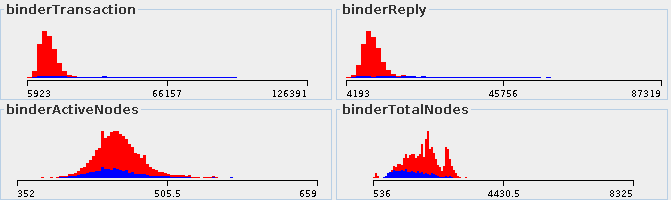
\includegraphics[width=\linewidth]{./poster/weka.png}
  \begin{itemize}\item A \item B \item C\end{itemize}
}


\headerbox{{\it Results} TODO}
{name=results,column=2,row=0,span=2}{
    \begin{center}
    {\small
    \newcommand{\resrow}[9]{#1 & #3 & #4 & #5 & #6 & #7 & #8 \\}
    \begin{tabular}{c|ccc|ccc}
        &
        \multicolumn{3}{|c|}{\bf Cross Validation} &
        \multicolumn{3}{c}{\bf Testing Set} \\
    \resrow{Classifier}{Size}
        {Correctly Classified}{TPR}{FPR}
        {Correctly Classified}{TPR}{FPR}{Time} \hline
    \resrow{Random Forest}{804K}
        {94.53\%}{97.66\%}{14.85\%}
        {70.31\%}{66.67\%}{26.90\%}{0m 0.647s}
    \resrow{Naive Bayes}{17K}
        {79.79\%}{87.85\%}{44.36\%}
        {78.91\%}{95.50\%}{33.79\%}{0m 0.261s}
    \resrow{Multilayer Perceptron}{2.7M}
        {93.91\%}{97.27\%}{16.13\%}
        {70.31\%}{61.26\%}{22.76\%}{0m 0.728s}
    \resrow{Bayes net}{2.7M}
        {86.23\%}{93.95\%}{36.88\%}
        {81.25\%}{97.30\%}{31.03\%}{0m 0.685s}
    \resrow{Logistic}{27K}
        {89.52\%}{97.07\%}{33.08\%}
        {68.75\%}{48.65\%}{15.86\%}{0m 0.268s}
    \resrow{J48}{77K}
        {93.43\%}{96.09\%}{14.55\%}
        {73.44\%}{72.97\%}{26.21\%}{0m 0.320s}
    \end{tabular}
    }
    \end{center}
    \begin{multicols}{2}
      \begin{itemize}\item A \item B \item C \item D \item E\end{itemize}
    \end{multicols}
}


\headerbox{TODO}
    {name=benign,column=2,below=results,above=bottom}{
  \begin{itemize}\item A \item B \item C \item D \item E\end{itemize}
}

\headerbox{TODO}
    {name=malicious,column=3,below=results,above=bottom}{
  \begin{itemize}\item A \item B \item C \item D \item E\end{itemize}
}

\end{poster}
\end{document}
